\chapter{Podaci i metode binarne klasifikacije} % Main chapter title
\label{Chapter3}

U ovom poglavlju biće opisani korišćeni podaci i način njihovog predstavljanja u račnuaru. Zatim će ukratko biti opisane metode binarne klasifikacije koje su korišćene za predviđanje funkcija proteina.


\section{Podaci}

Podaci o proteinima mogu se pronaći u biomedicinskim bazama podataka, a neke od njih prikazane su u tabeli \ref{tab: databases}. 

\begin{table}[H]
	\centering
	\begin{tabular}{|l|l|l|}
		\hline
		Baza podataka & URL & Opis \\
		\hline
		UniProtKB & \url{uniprot.org} & Proteinske sekvence i \\ & & funkcije proteina \\
		\hline
		PFAM & \url{pfam.xfam.org} & Proteinske familije \\
		\hline
		PDB & \url{wwpdb.org} & Eksperimentalno utvrđene strukture \\
		\hline
		ModBase & \url{modbase.compbio.ucsf.edu} & Strukture utvrđene predviđanjem \\
		\hline
		I2D & \url{ophid.utoronto.ca} & Interakcije između proteina \\
		\hline
		GEO & \url{www.ncbi.nlm.nih.gov/geo} & Podaci o genskoj ekspresiji \\
		\hline
		PRIDE & \url{www.ebi.ac.uk/pride} & Podaci dobijeni \\
		& & masenom sprektometrijom \\
		\hline 
	\end{tabular}
	\caption{Prikaz nekih javno dostupni biomedicinskih baza \\ podataka \cite{radivojac, doktJK}.}
	\label{tab: databases}
\end{table}



\subsection{Predstavljanje proteina}

% predstavljanje proteina preko sekvenci aminokiselina

Kao što je već rečeno, proteini su izgrađeni od 20 različitih aminokiselina, a svaka aminokiselina ima jedinstveni simbol (tabela \ref{tab: aminoacids}). Najjednostavniji način za predstavljanje proteina u računaru jeste kao niska karaktera nad azbukom $\Sigma = \{A, C, D, E, F,$ \\ $ G, H, I, K, L, M, N, P, Q, R, S, T, V, W, Y\}$. Nad ovako predstavljenim proteinima mogu su koristiti algoritmi za rad sa tekstom kao što je poravnanje sekvenci. \cite{radivojac}


\subsection{Predstavljanje funkcije proteina}

Da bi predviđanje funkcija proteina bilo moguće neophodno je da postoji kontrolisan rečnik i dobro definisani odnosi između funkcija. Sistem za predstavljanje funkcije proteina koji se trenutno najviše koristi je \textit{Gene Ontology}. Ovaj sistem deli funkcije proteina na tri ontologije: biološki procesi (BPO), molekulske funkcije (MFO) i ćelijske komponente (CCO). 


Svaka ontologija predstavljena je kao usmereni aciklički graf gde su čvorovima pridruženi nazivi funkcija, a grane koje ih povezuju definišu relaciju ‚‚is\_a''. Hijerarhijska organizacija obezbeđuje da svaki čvor ima specifičniju funkciju od roditeljskog čvora. Međutim, hijerarhija nije striktna zbog čega jedan čvor može imati više roditeljskih čvorova. U korenu svake ontologije nalazi se funkcija sa nazivom te ontologije, a u listovima su najspecifičnije fukcije. Na slici \ref{fig:subgraph} prikazan je podgraf ontologije molekulskih funkcija. \cite{doktJK, GO}


\begin{figure}[h]
	\centering
	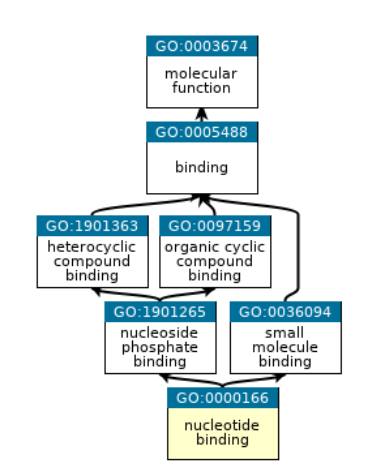
\includegraphics[width=0.6\textwidth]{Figures/go_subgraph.png}
	\caption{Prikaz podgrafa ontologije molekulskih funkcija za funkciju ‚‚nucleotid binding''.}
	\label{fig:subgraph}
\end{figure}


\section{Binarni klasifikatori}

Klasifikacija, odnosno, zadatak dodeljivanja objekata jednoj od više predefinisanih kategorija, rasprostranjen je problem koji obuhvata mnoštvo različitih primena. Primeri uključuju otkrivanje spam poruka na osnovu zaglavlja poruke i njenog sadržaja, kategorisanje ćelija kao maligne ili beningne na osnovu rezultata magnetne rezonance, klasifikacija galaksija na osnovu njihovog oblika, itd. Binarna klasifikacija je slučaj klasifikacije u kojoj postoje tačno dve predefinisane kategorije u koje treba razvrstati date objekte. Obično se za jednu kategoriju kaže da je to pozitivna klasa, a za drugu da je negativna.

Svaki klasifikator upotrebljava algoritam za učenje kako bi odredio model koji najbolje odgovara vezi između skupa atributa i klase ulaznih podataka. Model koji algoritam generiše trebalo bi da odgovara ulaznim podacima kao i da tačno predviđa klasu slogova koje ranije nije video. 


\iffalse 

\paragraph{Metod potpornih vektora} Ova tehnika predstavlja granicu odlučivanja podskupom trening instanci koje se nazivaju potporni vektori.  Dobro radi sa visokodimenzionalnim podacima i izbegava prokletsvo dimenzionalnosti.


\paragraph{Logistička regresija} Logistička regresija je statistički zasnovan metod za analizu skupa podataka u kom jedna ili više nezavisnih promenljivih određuju ishod. Određeni objekat ima veću verovatnoću da pripada pozitivnoj klasi što je više udaljen od hiperravni sa pozitivne strane, odnosno, veća je verovatnoća da pripada negativnoj klasi što je dalje od hiperravni sa njene negativne strane.


\paragraph{Slučajne šume} Metod slučajne šume spada u grupu metoda specijalno dizajnirane za stabla odlučivanja. Ona kombinuje predviđanja više različitih stabala, gde je svako stablo generisano na osnovu vrednosti nezavisnog skupa slučajno odabranih vektora. 



\fi 